\documentclass[tikz,border=8pt]{standalone}
% Shared look for every TikZ diagram. Load with \input{../../tools/tikz-style.tex}
\usepackage[T1]{fontenc}
\usepackage{lmodern}
\renewcommand{\sfdefault}{lmr}  % diagrams use the same serif as the text
\usetikzlibrary{arrows.meta, positioning, shapes.geometric, calc, fit, backgrounds}
\definecolor{cblue}{HTML}{4C78A8}
\definecolor{corange}{HTML}{F58518}
\definecolor{cgreen}{HTML}{54A24B}
\definecolor{cred}{HTML}{E45756}
\definecolor{cpurple}{HTML}{B279A2}
\definecolor{cgrey}{HTML}{6B6B6B}
\tikzset{
  every picture/.style={font=\sffamily, line width=1.2pt},
  box/.style={draw=#1, fill=#1!12, rounded corners=4pt, align=center, inner sep=7pt, minimum height=1.1cm},
  box/.default=cgrey,
  arrow/.style={-{Stealth[length=3mm]}, draw=cgrey, line width=1.4pt},
  title/.style={font=\sffamily\bfseries\Large},
  note/.style={font=\sffamily\small, text=cgrey, align=center},
}
\AtBeginDocument{\hyphenpenalty=10000 \exhyphenpenalty=10000}

\usetikzlibrary{matrix}
\begin{document}
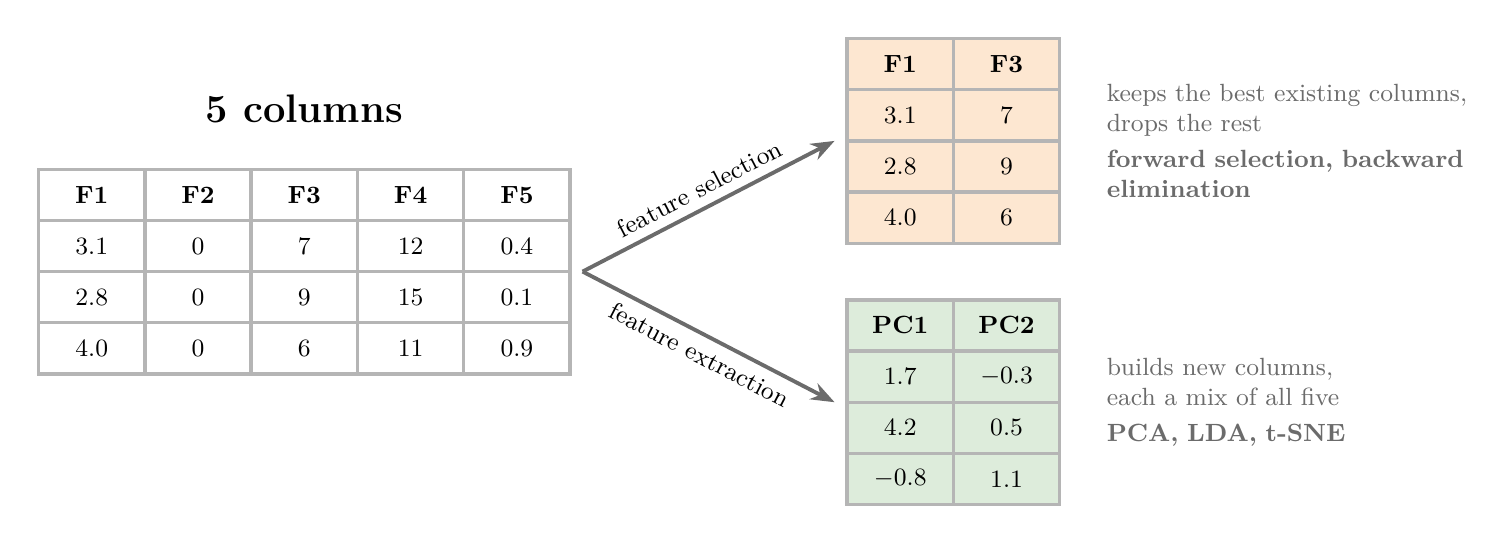
\begin{tikzpicture}
  \tikzset{tbl/.style={matrix of nodes, column sep=-\pgflinewidth, row sep=-\pgflinewidth,
           nodes={minimum width=1.35cm, minimum height=0.65cm, anchor=center, draw=cgrey!50, font=\small},
           row 1/.style={nodes={font=\small\bfseries}}}}
  % original table
  \matrix (a) [tbl] { F1 & F2 & F3 & F4 & F5 \\ 3.1 & 0 & 7 & 12 & 0.4 \\ 2.8 & 0 & 9 & 15 & 0.1 \\ 4.0 & 0 & 6 & 11 & 0.9 \\ };
  \node[title, above=0.3cm of a] {5 columns};
  % selection
  \matrix (s) [tbl, above right=0.2cm and 3.2cm of a.east, column 1/.style={nodes={fill=corange!20}},
               column 2/.style={nodes={fill=corange!20}}] { F1 & F3 \\ 3.1 & 7 \\ 2.8 & 9 \\ 4.0 & 6 \\ };
  % extraction
  \matrix (x) [tbl, below right=0.2cm and 3.2cm of a.east, nodes={fill=cgreen!20}] { PC1 & PC2 \\ 1.7 & $-$0.3 \\ 4.2 & 0.5 \\ $-$0.8 & 1.1 \\ };
  \draw[arrow] (a.east) -- (s.west) node[midway, above, sloped, font=\sffamily\small] {feature selection};
  \draw[arrow] (a.east) -- (x.west) node[midway, below, sloped, font=\sffamily\small] {feature extraction};
  \node[note, right=0.3cm of s, text width=4.6cm, align=left] {keeps the best existing columns,\\drops the rest\\[2pt] \textbf{forward selection, backward elimination}};
  \node[note, right=0.3cm of x, text width=4.6cm, align=left] {builds new columns,\\each a mix of all five\\[2pt] \textbf{PCA, LDA, t-SNE}};
\end{tikzpicture}
\end{document}
